\notename
\chap{ỨNG DỤNG CỦA ĐẠO HÀM}
\section{SỰ ĐỒNG BIẾN, NGHỊCH BIẾN CỦA HÀM SỐ}
\Opensolutionfile{ans}[ans/ansCD2D1-1]
\subsection{Tóm tắt lý thuyết}
\subsubsection{Định nghĩa}
Cho hàm số $f(x)$ xác định trên khoảng (đoạn hoặc nửa khoảng) $K$.
\begin{center}
	\begin{itemize}
	\item Hàm số $f$ gọi là đồng biến (tăng) trên $K$ nếu với mọi cặp $x_1,x_2\in K$ mà $x_1<x_2\Rightarrow f(x_1)<f(x_2)$.
	\item Hàm số $f$ gọi là nghịch biến (giảm) trên $K$ nếu với mọi cặp $x_1,x_2\in K$ mà $x_1<x_2\Rightarrow f(x_1)>f(x_2)$.
	\end{itemize}
\end{center}
\begin{note}
Hàm số đồng biến hoặc nghịch biến trên $K$ (với $K$ là một khoảng (đoạn), nửa khoảng) được gọi chung là hàm số đơn điệu trên $K$.	
\end{note}
\subsubsection{Mối quan hệ giữa tính đơn điệu của hàm số và dấu của đạo hàm}
\begin{enumerate}
	\item {\bf Điều kiện cần để hàm số đơn điệu}\\ 
	Giả sử hàm số $f(x)$ có đạo hàm trên khoảng $I$. Khi đó
	\begin{itemize}
	\item Nếu hàm số $f(x)$ đồng biến trên $I$ thì $f'(x)\geq 0,\forall x\in I$.
	\item Nếu hàm số $f(x)$ nghịch biến trên $I$ thì $f'(x)\leq 0,\forall x\in I$.
	\end{itemize}
 	\item {\bf Điều kiện đủ để hàm số đơn điệu}\\
 	Giả sử hàm số $f(x)$ có đạo hàm trên khoảng $I$.
 	\begin{itemize}
 	\item Nếu $f'(x)\geq 0,\forall x\in I$ và $f'(x)=0$ tại một số hữu hạn điểm của $I$ thì hàm số đồng biến trên $I$.
 	\item Nếu $f'(x)\leq 0,\forall x\in I$ và $f'(x)=0$ tại một số hữu hạn điểm của $I$ thì hàm số nghịch biến trên $I$.
 	\item Nếu $f'(x)=0,\forall x\in I$ thì hàm số không đổi trên $I$.
 	\end{itemize}
 \item Giả sử hàm số $f(x)$ liên tục trên nửa khoảng $[a;b)$ và có đạo hàm trên khoảng $(a;b)$.
\begin{itemize}
	\item Nếu $f'(x)>0$ (hoặc $f'(x)<0$) với mọi $x\in(a;b)$ thì hàm số đồng biến (hoặc nghịch biến) trên nửa khoảng $[a;b)$.
	\item Nếu $f'(x)=0,\forall x\in(a;b)$ thì hàm số $f$ không đổi trên nửa khoảng $[a;b)$.
\end{itemize}
\item Nếu hàm số đồng biến trên K thì đồ thị hàm số là một đường đi lên từ trái sang phải trên K.\\
Nếu hàm số nghịch biến trên K thì đồ thị hàm số là một đường đi xuống từ trái sang phải.
\begin{center}
	\begin{minipage}{0.45\textwidth}
	\begin{tikzpicture}[>=stealth,scale=0.5]
	\draw[->] (-1,0)--(6,0) node[below]{$x$};
	\draw[->] (0,-1)--(0,6) node[right]{$y$};
	\draw [domain=2:5,blue,very thick,samples=100] plot (\x,{0.25*(\x-2)^2+1});
	\draw[dashed](2,0)node[below]{$x_1$}--(2,1)--(0,1)node[left]{$f(x_1)$};
	\draw[dashed](5,0)node[below]{$x_2$}--(5,13/4)--(0,13/4)node[left]{$f(x_2)$};
	\draw (4,4) node[above]{\fbox{Hàm số đồng biến}};
	\end{tikzpicture}
	\end{minipage}
	\begin{minipage}{0.45\textwidth}
	\begin{tikzpicture}[>=stealth,scale=0.5]
	\draw[->] (-1,0)--(6,0) node[below]{$x$};
	\draw[->] (0,-1)--(0,6) node[right]{$y$};
	\draw [domain=2:5,red,very thick,samples=100] plot (\x,{-0.25*(\x-2)^2+3});
	\draw[dashed](2,0)node[below]{$x_1$}--(2,3)--(0,3)node[left]{$f(x_1)$};
	\draw[dashed](5,0)node[below]{$x_2$}--(5,3/4)--(0,3/4)node[left]{$f(x_2)$};
	\fill (4,4) node[above]{\fbox{Hàm số nghịch biến}};
	\end{tikzpicture}
	\end{minipage}
\end{center}
\end{enumerate}
\newpage
\subsection{Phân loại và phương pháp giải bài tập}
\begin{dang}{Xét tính đơn điệu của hàm số cho bởi công thức}.
\dotlineEX{3}
\end{dang}
\subsubsection{Các ví dụ}
\begin{vd}%[2D1B1-2]%Câu 1.
	Tìm các khoảng đồng biến, nghịch biến của hàm số $y=\dfrac{x+1}{x+3}$.
	\loigiai{
	Tập xác định $\mathscr{D}=\mathbb{R}\setminus\{-3\}$.\\
	$y'=\dfrac{2}{(x+3)^2}>0,\forall x\neq-3$.\\
	Do đó hàm số đồng biến trên các khoảng $(-\infty;-3)$ và $(-3;+\infty)$.}
\end{vd}
\begin{vd}%[2D1B1-2]%Câu 2.
	Xét tính đơn điệu của hàm số $y=2x^3+6x^2+6x-7$.
	\loigiai{
	Tập xác định $\mathscr{D}=\mathbb{R}$.\\
	$y'=6x^2+12x+6=6(x+1)^2\geq 0,\forall x\in\mathbb{R}$.\\
	Do đó hàm số đồng biến trên $\mathbb{R}$.}
\end{vd}
\begin{vd}%[2D1B1-2]%Câu 3.
	Tìm khoảng đồng biến của hàm số $y=\dfrac{x}{x^2+1}$.
	\loigiai{
	Tập xác định $\mathscr{D}=\mathbb{R}$.\\
	$y'=\dfrac{x^2+1-2x^2}{\left(x^2+1\right)^2}=\dfrac{1-x^2}{\left(x^2+1\right)^2}$; $y'=0\Rightarrow 1-x^2=0\Leftrightarrow\hoac{&x=1\\&x=-1.}$ \\
	Bảng biến thiên
	\begin{center}
	\begin{tikzpicture}[scale=1, font=\footnotesize, line join=round, line cap=round, >=stealth]
	\tkzTabInit[nocadre=false,lgt=1,espcl=2.5,deltacl=0.5]{$x$/.7 ,$y'$/.7,$y$/2}
	{$-\infty$ , $-1$ , $1$ , $+\infty$}
	\tkzTabLine{ , - , $0$ , + , $0$ , - , }
	\tkzTabVar{+/$0$ , -/$-\dfrac{1}{2}$ , +/$\dfrac{1}{2}$ , -/$0$}
	\end{tikzpicture}
	\end{center}
	Hàm số đồng biến trên khoảng $(-1;1)$.}
\end{vd}
\begin{vd}%[2D1B1-2]%Câu 4.
	Tìm các khoảng đơn điệu của hàm số $y=\sqrt{2x-x^2}$.
	\loigiai{
	Tập xác định $\mathscr{D}=[0; 2]$.\\
	Ta có $y'=\dfrac{1-x}{\sqrt{2x-x^2}}$.\\
	Lập bảng biến thiên. 
	\begin{center}
	\begin{tikzpicture}[scale=1, font=\footnotesize, line join=round, line cap=round, >=stealth]
\tkzTabInit[nocadre=false,lgt=1,espcl=3,deltacl=0.5]{$x$/.7 ,$y'$/.7,$y$/2}
{$0$ , $1$ , $2$}
\tkzTabLine{ , + , $0$ , - , }
\tkzTabVar{-/$0$ , +/$1$ , -/$0$}
\end{tikzpicture}	
	\end{center}
	Do đó hàm số đồng biến trên khoảng $(0;1)$ và nghịch biến trên khoảng $(1;2)$.}
\end{vd}
\begin{vd}%[2D1B1-2]%Câu 5.
	Tìm khoảng đồng biến của hàm số $y=f(x)$ liên tục trên $\mathbb{R}$ và có đạo hàm $f'(x)=(x+1)^2(2-x)(x+3)$.
	\loigiai{
	Ta có $f'(x)=(x+1)^2(2-x)(x+3)=0\Leftrightarrow\hoac{&x=-1\\&x=2\\&x=-3.}$\\
	Bảng biến thiên
	\begin{center}
	\begin{tikzpicture}[scale=1, font=\footnotesize, line join=round, line cap=round, >=stealth]
	\tkzTabInit[nocadre=false,lgt=1.2,espcl=2,deltacl=0.5]{$x$/.7 ,$f'(x)$/.7,$f(x)$/2}
	{$-\infty$ , $-3$ , $-1$ , $2$ , $+\infty$}
	\tkzTabLine{ , - , $0$ , + , $0$ , + , $0$ , - , }
	\coordinate (3) at ($(N53)+(0,.2)$);
	\node (0) at ($(N12)-(0,.2)$){$+\infty$};
	\node (1) at ($(N23)+(0,.2)$){$f(-3)$};
	\node (2) at ($(N42)-(0,.2)$){$f(2)$};
	\node (3) at ($(N53)+(0,.2)$){$-\infty$};
	\draw[-stealth] (0)--(1);
	\draw[-stealth] (1)--(2);
	\draw[-stealth] (2)--(3);
	\end{tikzpicture}
	\end{center}
	Vậy hàm số đồng biến trên khoảng $(-3;2)$.}
\end{vd}
\subsubsection{Câu hỏi trắc nghiệm}
\begin{ex}%[Nguyễn Cường - ĐCHT THPT]%[2D1B1-1]%Câu 1.
	Cho hàm số $y=x^2\left(6-x^2\right)$. Khẳng định nào sau đây là \textbf{đúng}?
	\choice
	{\True Hàm số đồng biến trên $\left(-\infty;-\sqrt{3}\right)$ và $(0;\sqrt{3})$}
	{Hàm số nghịch biến trên $\left(-\sqrt{3};0\right)\cup\left(\sqrt{3};+\infty\right)$}
	{Hàm số đồng biến trên $(-\infty;-3)$ và $(0;3)$}
	{Hàm số đồng biến trên $(-\infty;9)$}
	\loigiai{
	Tập xác định $\mathscr{D}=\mathbb{R}$.\\
	Ta có $y=-x^4+6x^2$ nên $y'=-4x^3+12x$.\\
	$y'=0\Leftrightarrow\hoac{&x=0\\&x=\pm\sqrt{3}.}$ \\
	Bảng biến thiên
	\begin{center}
	\begin{tikzpicture}[scale=1, font=\footnotesize, line join=round, line cap=round, >=stealth]
	\tkzTabInit[nocadre=false,lgt=1,espcl=2.5,deltacl=0.5]{$x$/.7 ,$y'$/.7,$y$/2}
	{$-\infty$ , $-\sqrt{3}$ , $0$ , $\sqrt{3}$ , $+\infty$}
	\tkzTabLine{ , + , $0$ , - , $0$ , + , $0$ , - , }
	\tkzTabVar{-/$-\infty$ , +/$9$, -/$0$ , +/$9$ , -/$-\infty$}
	\end{tikzpicture}
	\end{center}
	Hàm số đồng biến trên $\left(-\infty;-\sqrt{3}\right)$ và $(0;\sqrt{3})$.}
\end{ex}
\begin{ex}%[Nguyễn Cường - ĐCHT THPT]%[2D1B1-1]%Câu 2.
	Cho hàm số $y=\dfrac{2x+5}{x+1}$. Khẳng định nào sau đây đúng?
	\choice
	{Hàm số đồng biến trên $\mathbb{R}\setminus\{-1\}$}
	{\True Hàm số nghịch biến trên các khoảng $(-\infty;-1);(-1;+\infty)$}
	{Hàm số nghịch biến trên $\mathbb{R}\setminus\{-1\}$}
	{Hàm số nghịch biến trên các khoảng $(-\infty;-1);(-1;+\infty)$}
	\loigiai{
	Tập xác định $\mathscr{D}=\mathbb{R}\setminus\{-1\}$.\\
	Ta có $y'=\dfrac{-3}{(x+1)^2}<0,\forall x\neq-1$.\\
	Do đó hàm số nghịch biến trên các khoảng $(-\infty;-1);(-1;+\infty)$.}
\end{ex}
\begin{ex}%[Nguyễn Cường - ĐCHT THPT]%[2D1B1-1]%Câu 3.
	Hàm số $y=\dfrac{2}{2+x^2}$ đồng biến trên khoảng nào dưới đây?
	\choice
	{$(-2;2)$}
	{$(0;+\infty)$}
	{\True $(-\infty;0)$}
	{$(-\infty;+\infty)$}
	\loigiai{
	Tập xác định $\mathscr{D}=\mathbb{R}$
	$y'=-\dfrac{4x}{\left(2+x^2\right)^2}$\\
	$y'=0\Leftrightarrow x=0$.
	\begin{center}
	\begin{tikzpicture}[scale=1, font=\footnotesize, line join=round, line cap=round, >=stealth]
	\tkzTabInit[nocadre=false,lgt=1,espcl=3,deltacl=0.5]{$x$/.7 ,$y'$/.7,$y$/2}
	{$-\infty$ , $x0$ , $+\infty$}
	\tkzTabLine{ , + , $0$ , - , }
	\tkzTabVar{-/$0$ , +/$1$ , -/$0$}
	\end{tikzpicture}
	\end{center}
	Do đó hàm số đồng biến trên $(-\infty;0)$.}
\end{ex}
\begin{ex}%[Nguyễn Cường - ĐCHT THPT]%[2D1B1-1]%Câu 4.
	Cho hàm số $y=f(x)$ có đạo hàm $f'(x)=3x^2+2,\forall x\in\mathbb{R}$. Mệnh đề nào sau đây \textbf{đúng}?
	\choice
	{Hàm số nghịch biến trên khoảng $(3;+\infty)$}
	{Hàm số nghịch biến trên khoảng $(-\infty;1)$}
	{\True Hàm số đồng biến trên khoảng $(-\infty;+\infty)$}
	{Hàm số nghịch biến trên khoảng $(1;3)$}
	\loigiai{
	Tập xác định $\mathscr{D}=\mathbb{R}$.\\
	Ta có $f'(x)=3x^2+2>0,\forall x\in\mathbb{R}$, suy ra hàm số đồng biến trên khoảng $(-\infty;+\infty)$.}
\end{ex}
\begin{ex}%[Nguyễn Cường - ĐCHT THPT]%[2D1B1-1]%Câu 5.
	Hàm số $y=x^3-3x+1$ nghịch biến trên khoảng nào trong các khoảng sau?
	\choice
	{\True $(-1;1)$}
	{$(-\infty;-1)$}
	{$(1;+\infty)$}
	{$(-1;3)$}
	\loigiai{
	Tập xác định $\mathscr{D}=\mathbb{R}$.\\
	Ta có $y'=3x^2-3$.\\
	$y'=0\Leftrightarrow 3x^2-3=0\Leftrightarrow\hoac{&x=1\\&x=-1}$ 
	\begin{center}
	\begin{tikzpicture}[scale=1, font=\footnotesize, line join=round, line cap=round, >=stealth]
	\tkzTabInit[nocadre=false,lgt=1,espcl=2.5,deltacl=0.5]{$x$/.7 ,$y'$/.7,$y$/2}
	{$-\infty$ , $-1$ , $1$ , $+\infty$}
	\tkzTabLine{ , + , $0$ , - , $0$ , + , }
	\tkzTabVar{-/$-\infty$ , +/$3$ , -/$1$ , +/$+\infty$}
	\end{tikzpicture}
	\end{center}
	Dựa vào BBT ta thấy hàm số nghịch biến trên $(-1;1)$.}
\end{ex}
\begin{ex}%[Nguyễn Cường - ĐCHT THPT]%[2D1B1-1]%Câu 6.
	Hàm số nào dưới đây đồng biến trên $\mathbb{R}$?
	\choice
	{$y=x^2+1$}
	{\True $y=2x+1$}
	{$y=-2x+1$}
	{$y=-x^2+1$}
	\loigiai{
	Hàm số $y=2x+1$ có $y'=2>0,\forall x\in\mathbb{R}$ nên hàm số $y=2x+1$ đồng biến trên $\mathbb{R}$.}
\end{ex}
\begin{ex}%[Nguyễn Cường - ĐCHT THPT]%[2D1B1-1]%Câu 7.
	Cho hàm số $y=\sqrt{x^2-1}$. Mệnh đề nào dưới đây đúng?
	\choice
	{Hàm số nghịch biến trên $(-\infty;0)$}
	{Hàm số đồng biến trên $(0;+\infty)$}
	{Hàm số đồng biến trên $(-\infty;+\infty)$}
	{\True Hàm số đồng biến trên $(1;+\infty)$}
	\loigiai{
	Tập xác định $\mathscr{D}=(-\infty;-1]\cup[1;+\infty)$.\\
	$y'=\dfrac{1}{2\sqrt{x^2-1}}\left(x^2-1\right)'=\dfrac{x}{\sqrt{x^2-1}}$ 
	\begin{center}
	\begin{tikzpicture}[scale=1, font=\footnotesize, line join=round, line cap=round, >=stealth]
\tkzTabInit[nocadre=false,lgt=1,espcl=3,deltacl=0.5]{$x$/.7 ,$y'$/.7,$y$/2}
{$-\infty$, $-1$, $1$, $+\infty$}
\tkzTabLine{, -,d , h, d, +, }
\tkzTabVar{+/$+\infty$ , -H/$0$, -/$0$,+/$+\infty$}
\node (0) at ($(N21)!.5!(N31)+(0,.35)$){$0$};
\end{tikzpicture}
	\end{center}
	Vậy hàm số đồng biến trên $(1;+\infty)$.}
\end{ex}
\begin{ex}%[Nguyễn Cường - ĐCHT THPT]%[2D1B1-1]%Câu 8.
	Hàm số $y=\sqrt{2x-x^2}$ đồng biến trên khoảng
	\choice
	{$(1;2)$}
	{$(-\infty;1)$}
	{$(1;+\infty)$}
	{\True $(0;1)$}
	\loigiai{
	Tập xác định $\mathscr{D}=[0;2]$.\\ $y'=\dfrac{1-x}{\sqrt{2x-x^2}}=0\Leftrightarrow x=1\Rightarrow y=1$.\\
	Bảng biến thiên
	\begin{center}
	\begin{tikzpicture}[>=stealth]
	\tkzTabInit[nocadre=false,lgt=1,espcl=3,deltacl=0.5]{$x$/.7 ,$y'$/.7,$y$/2}
	{$0$ , $1$ , $2$}
	\tkzTabLine{ d, + , $0$ , - ,d }
	\tkzTabVar{-/$0$ , +/$1$ , -/$0$}
	\end{tikzpicture}
	\end{center}
	Vậy hàm số $y=\sqrt{2x-x^2}$ đồng biến trên khoảng $(0;1)$.}
\end{ex}
\begin{ex}%[Nguyễn Cường - ĐCHT THPT]%[2D1B1-1]%Câu 9.
	Hàm số $y=\dfrac{x}{x^2+1}$ đồng biến trên khoảng nào sau đây?
	\choice
	{$(-\infty;-1)$}
	{$(0;+\infty)$}
	{$(-\infty;+\infty)$}
	{\True $(-1;1)$}
	\loigiai{
	Tập xác định $\mathscr{D}=\mathbb{R}$.\\
	Ta có $y'=\dfrac{1-x^2}{\left(1+x^2\right)^2}\Rightarrow y'=0\Leftrightarrow x=\pm 1$.\\
	Bảng biến thiên
	\begin{center}
	\begin{tikzpicture}[scale=1, font=\footnotesize, line join=round, line cap=round, >=stealth]
	\tkzTabInit[nocadre=false,lgt=1,espcl=2.5,deltacl=0.5]{$x$/.7 ,$y'$/.7,$y$/2}
	{$-\infty$ , $-1$ , $1$ , $+\infty$}
	\tkzTabLine{ , - , $0$ , + , $0$ , - , }
	\tkzTabVar{+/$0$ , -/$-\dfrac{1}{2}$ , +/$\dfrac{1}{2}$ , -/$0$}
	\end{tikzpicture}
	\end{center}
	Vậy hàm số đồng biến trên khoảng $(-1;1)$.}
\end{ex}
\begin{ex}%[Nguyễn Cường - ĐCHT THPT]%[2D1B1-1]%Câu 10.
	Cho hàm số $y=\dfrac{3x+2}{x-1}$. Mệnh đề nào sau đây đúng?
	\choice
	{Hàm số nghịch biến trên $\mathbb{R}\setminus\{1\}$}
	{Hàm số đồng biến trên $\mathbb{R}\setminus\{1\}$}
	{\True Hàm số nghịch biến trên các khoảng $(-\infty;1)$ và $(1;+\infty)$}
	{Hàm số đồng biến trên các khoảng $(-\infty;1)$ và $(1;+\infty)$}
	\loigiai{
	Tập xác định $\mathscr{D}=\mathbb{R}\setminus\{1\}$.\\
	Ta có $y'=\dfrac{-5}{(x-1)^2}<0 , \forall x \in \mathscr{D}$.\\
	Vậy hàm số nghịch biến trên các khoảng $(-\infty;1)$ và $(1;+\infty)$. }
\end{ex}
\begin{ex}%[Nguyễn Cường - ĐCHT THPT]%[2D1B1-1]%Câu 11.
	Cho hàm số $f(x)=\sin x-\cos x+2x$. Khẳng định nào sau đây là đúng?
	\choice
	{\True Hàm số $y=f(x)$ đồng biến trên $\mathbb{R}$}
	{Hàm số $y=f(x)$ là hàm số lẻ trên $\mathbb{R}$}
	{Hàm số $y=f(x)$ nghịch biến trên $(-\infty; 0)$}
	{Hàm số $y=f(x)$ nghịch biến trên $\left(0;\dfrac{\pi}{2}\right)$}
	\loigiai{
	Tập xác định $\mathscr{D}=\mathbb{R}$.\\
	$f'(x)=\cos x+\sin x+2=\sqrt{2}\sin\left(x+\dfrac{\pi}{4}\right)+2$.\\
	Do $\sin\left(x+\dfrac{\pi}{4}\right)\geq-1, \forall x \in \mathbb{R}$ nên$ f'(x)\geq-\sqrt{2}+2>0, \forall x\in\mathbb{R}$.\\
	Vậy hàm số đồng biến trên $\mathbb{R}$.}
\end{ex}
\begin{ex}%[Nguyễn Cường - ĐCHT THPT]%[2D1B1-1]%Câu 12.
	Cho các hàm số $y=\dfrac{x+1}{x+2}$, $y=\tan x$, $y=x^3+x^2+4x-2017$. Có bao nhiêu hàm số đồng biến trên $\mathbb{R}$?
	\choice
	{$0$}
	{$3$}
	{\True $1$}
	{$2$}
	\loigiai{
	Ta có hàm số đồng biến trên $\mathbb{R}$ nên tập xác định $\mathscr{D}=\mathbb{R}$.\\
	Suy ra loại hai hàm số $y=\dfrac{x+1}{x+2}$, $y=\tan x$.\\
	Xét hàm số $y=x^3+x^2+4x-2017$ có tập xác định $\mathscr{D}=\mathbb{R}$ và $y'=3x^2+2x+4>0,\forall x\in\mathbb{R}$ suy ra hàm số đồng biến trên $\mathbb{R}$.}
\end{ex}
\begin{ex}%[Nguyễn Cường - ĐCHT THPT]%[2D1B1-1]%Câu 13.
	Hàm số nào sau đây có chiều biến thiên khác với chiều biến thiên của các hàm số còn lại. 
	\choice
	{$h(x)=x^3+x-\sin x$}
	{$k(x)=2x+1$}
	{$g(x)=x^3-6x^2+15x+3$}
	{\True $f(x)=\dfrac{-x^2-2x+5}{x+1}$}
	\loigiai{
	Ta có\\
	$f'(x)=\dfrac{-x^2-2x-7}{(x+1)^2}=\dfrac{-(x+1)^2-6}{(x+1)^2}<0,\forall x\neq-1\Rightarrow f(x)$ luôn nghịch biến trên từng khoảng xác định.\\
	$g'(x)=3x^2-12x+15=3(x-2)^2+3>0,\forall x\Rightarrow g(x)$ luôn đồng biến trên $\mathbb{R}$.\\
	$k'(x)=2>0,\forall x\Rightarrow k(x)$ luôn đồng biến trên $\mathbb{R}$.\\
	$h'(x)=3x^2+1-\cos x=3x^2+2\sin^2\dfrac{x}{2}\geq 0,\forall x\in\mathbb{R}$ và do hàm số $h(x)=x^3+x-\sin x$ liên tục trên $\mathbb{R}$ nên hàm số $h(x)$ đồng biến trên $\mathbb{R}$.\\
	Qua đây ta nhận thấy các hàm số $h(x)$, $g(x)$, $k(x)$ đồng biến trên $\mathbb{R}$, còn hàm $f(x)$ thì không.}
\end{ex}
\begin{ex}%[Nguyễn Cường - ĐCHT THPT]%[2D1B1-1]%Câu 14.
	Cho hàm số $y=\sin x-\cos x+\sqrt{3}x$. Tìm khẳng định đúng trong các khẳng định sau: 
	\choice
	{Hàm số nghịch biến trên $(-\infty;0)$}
	{Hàm số nghịch biến trên $(1;2)$}
	{Hàm số là hàm số lẻ}
	{\True Hàm số đồng biến trên $(-\infty;+\infty)$}
	\loigiai{
	Tập xác đinh $\mathscr{D}=\mathbb{R}$.\\
	$y'=\cos x+\sin x+\sqrt{3} =\sqrt{2}\sin\left(x+\dfrac{\pi}{4}\right)+\sqrt{3} =\sqrt{2}\left[\sin\left(x+\dfrac{\pi}{4}\right)+1\right]+\left(\sqrt{3}-\sqrt{2}\right) >0$.\\
	Vậy hàm số đồng biến trên $(-\infty;+\infty)$.}
\end{ex}
\begin{ex}%[Nguyễn Cường - ĐCHT THPT]%[2D1K1-1]%Câu 15.
	Cho hàm số $y=f(x)$ xác định trên $\mathbb{R}$ và có đạo hàm $f’(x)$ thỏa mãn $f’(x)=(1-x)(x+2)g(x)+2018$ với $g(x)<0, \forall x\in\mathbb{R}$. Hàm số $y=f(1-x)+2018x+2019$ nghịch biến trên khoảng nào?
	\choice
	{$(1;+\infty)$}
	{$(0;3)$}
	{$(-\infty;3)$}
	{\True $(3;+\infty)$}
	\loigiai{
	Ta có $y’=-f’(1-x)+2018=-\left[1-(1-x)\right]\left[(1-x)+2\right]g(1-x)-2018+2018$.\\
	$=-x(3-x)g(1-x)$.\\
	Suy ra $y’<0\Leftrightarrow x(3-x)<0\Leftrightarrow\hoac{&x<0\\&x>3}$ (do $g(1-x)<0, \forall x\in\mathbb{R}$).\\
	Vậy hàm số nghịch biến trên khoảng $(3;+\infty)$.}
\end{ex}
\begin{ex}%[Nguyễn Cường - ĐCHT THPT]%[2D1B1-1]%Câu 16.
	 Hàm số $y=\sqrt{x-x^2}$ nghịch biến trên khoảng
	\choice
	{\True $\left(\dfrac{1}{2}; 1\right)$}
	{$\left(0;\dfrac{1}{2}\right)$}
	{$(-\infty; 0)$}
	{$(1;+\infty)$}
	\loigiai{
	Tập xác định $\mathscr{D}=[0;1]$.\\
	Ta có $y'=\dfrac{-2x+1}{2\sqrt{x-x^2}}$.\\
	$y'=0\Leftrightarrow -2x+1=0 \Leftrightarrow x=\dfrac{1}{2}$.\\
	Bảng biến thiên 
	\begin{center}
	\begin{tikzpicture}[scale=1, font=\footnotesize, line join=round, line cap=round, >=stealth]
	\tkzTabInit[nocadre=false,lgt=1,espcl=2.5,deltacl=0.5]{$x$/.8 ,$y'$/.7,$y$/2}
	{$0$ , $\dfrac{1}{2}$ , $1$}
	\tkzTabLine{ d, + , $0$ , - ,d }
	\tkzTabVar{-/$0$ , +/$\dfrac{1}{2}$ , -/$0$}
	\end{tikzpicture}
	\end{center}
	Vậy hàm số nghịch biến trên $\left(\dfrac{1}{2};1\right)$.}
\end{ex}
\begin{ex}%[Nguyễn Cường - ĐCHT THPT]%[2D1B1-1]%Câu 17.
	Hỏi hàm số $y=\sqrt{x^2-4x+3}$ đồng biến trên khoảng nào?
	\choice
	{$(2;+\infty)$}
	{$(-\infty;3)$}
	{$(-\infty;1)$}
	{\True $(3;+\infty)$}
	\loigiai{
	Tập xác định $\mathscr{D}=(-\infty;1]\cup[3;+\infty)$.\\
	Ta có $y'=\dfrac{2x-4}{2\sqrt{x^2-4x+3}}=\dfrac{x-2}{\sqrt{x^2-4x+3}}$.\\
	$y'>0\Leftrightarrow x>2$, kết hợp điều kiện xác định thì hàm số đồng biến trên $(3;+\infty)$.}
\end{ex}
\begin{ex}%[Nguyễn Cường - ĐCHT THPT]%[2D1B1-1]%Câu 18.
	Cho hàm số $y=\dfrac{x}{2}+\sin^2x; x\in[0;\pi]$. Hỏi hàm số đồng biến trên các khoảng nào?
	\choice
	{\True $\left(0;\dfrac{7\pi}{12}\right)$ và $\left(\dfrac{11\pi}{12};\pi\right)$}
	{$\left(\dfrac{7\pi}{12};\dfrac{11\pi}{12}\right)$}
	{$\left(\dfrac{7\pi}{12};\dfrac{11\pi}{12}\right)$ và $\left(\dfrac{11\pi}{12};\pi\right)$}
	{$(3;+\infty)$}
	\loigiai{
	Tập xác định $\mathscr{D}=\mathbb{R}$.\\
	$y'=\dfrac{1}{2}+\sin 2x$. \\
	Giải $y'=0\Leftrightarrow\hoac{&x=\dfrac{-\pi}{12}+k\pi\\&x=\dfrac{7\pi}{12}+k\pi}(k\in\mathbb{Z})$.\\
	Vì $x\in[0;\pi]$ nên có $2$ giá trị $x=\dfrac{7\pi}{12}$ và $x=\dfrac{11\pi}{12}$ thỏa điều kiện.\\
	Bảng biến thiên
	\begin{center}
	\begin{tikzpicture}[scale=1, font=\footnotesize, line join=round, line cap=round, >=stealth]
	\tkzTabInit[nocadre=false,lgt=1,espcl=3,deltacl=0.5]{$x$/.8 ,$y'$/.7,$y$/2}
	{$0$ , $\dfrac{7\pi}{12}$ , $\dfrac{11\pi}{12}$ , $\pi$}
	\tkzTabLine{ , + , $0$ , - , $0$ , + , }
	\tkzTabVar{-/$0$ , +/$y\left(\dfrac{7\pi}{12}\right)$ , -/$y\left(\dfrac{11\pi}{12}\right)$ , +/$\dfrac{\pi}{2}$}
	\end{tikzpicture}	
	\end{center}
	Vậy hàm số đồng biến trên các khoảng $\left(0;\dfrac{7\pi}{12}\right)$ và $\left(\dfrac{11\pi}{12};\pi\right)$.
	}
\end{ex}
\begin{ex}%[Nguyễn Cường - ĐCHT THPT]%[2D1B1-1]%Câu 19.
	Trong các hàm số sau, hàm số nào đồng biến trên $\mathbb{R}$?
	\choice
	{$y=x^4+x^2-1$}
	{$y=\dfrac{x+1}{x+3}$}
	{$y=x^2+1$}
	{\True $y=x^3+x$}
	\loigiai{
	Xét hàm số $y=x^3+x$ có tập xác định $\mathscr{D}=\mathbb{R}$.\\
$y'=3x^2+1 >0, \, \forall x \in \mathbb{R}$.\\
Vậy hàm số đồng biến trên $\mathbb{R}$.}
\end{ex}
\begin{ex}%[Nguyễn Cường - ĐCHT THPT]%[2D1B1-1]%Câu 20.
	Cho hàm số $y=\dfrac{x-3}{x+3}$. Khẳng định nào sau đây là đúng?
	\choice
	{Hàm số đơn điệu trên $\mathbb{R}$}
	{\True Hàm số đồng biến trên các khoảng $(-\infty;-3)$ và $(-3;+\infty)$}
	{Hàm số nghịch biến trên}
	{Hàm số đồng biến trên}
	\loigiai{
	Tập xác định $\mathscr{D}=\mathbb{R}\setminus \{-3\}$.\\
	Ta có $y'=\dfrac{6}{(x+3)^2}>0 ,\, \forall x\in \mathscr{D}$.\\
	Do đó hàm số đồng biến trên các khoảng xác định.\\
	Vậy hàm số đồng biến trên các khoảng $(-\infty;-3)$ và $(-3;+\infty)$.}
\end{ex}
\Closesolutionfile{ans}